\vspace{-.15in}
\section{Evolution}
\label{sec:evolution}
\vspace{-.1in}

\begin{figure}[t!]
\centering
\begin{subfigure}[b]{.32\textwidth}
  \centering
  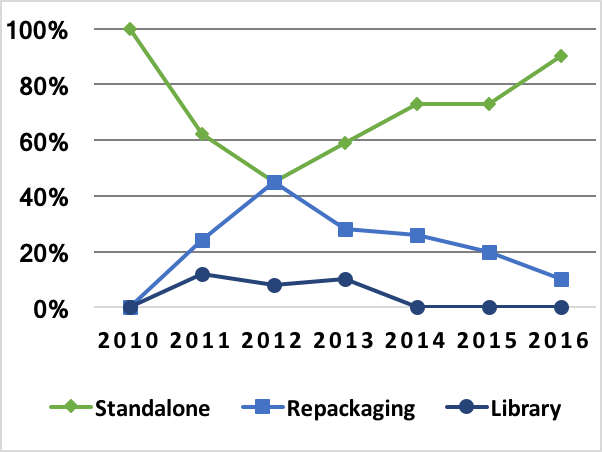
\includegraphics[width=0.9\linewidth]{fig/charts/comp.png}
  \caption{Composition}
  \label{fig:sub:ins}
\end{subfigure}%
\begin{subfigure}[b]{.32\textwidth}
  \centering
  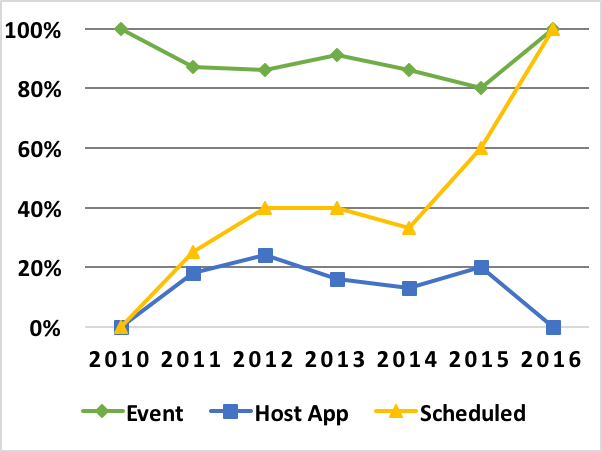
\includegraphics[width=0.9\linewidth]{fig/charts/act.png}
  \caption{Activation}
  \label{fig:sub:act}
\end{subfigure}%
\begin{subfigure}[b]{.32\textwidth}
  \centering
  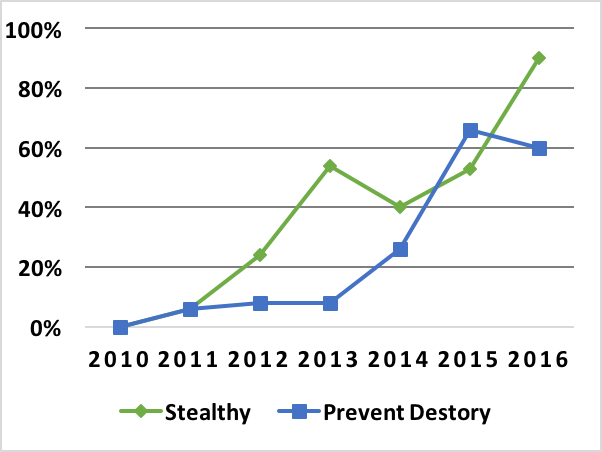
\includegraphics[width=0.9\linewidth]{fig/charts/per.png}
  \caption{Persistence}
  \label{fig:sub:per}
\end{subfigure}
\begin{subfigure}[b]{.32\textwidth}
  \centering
  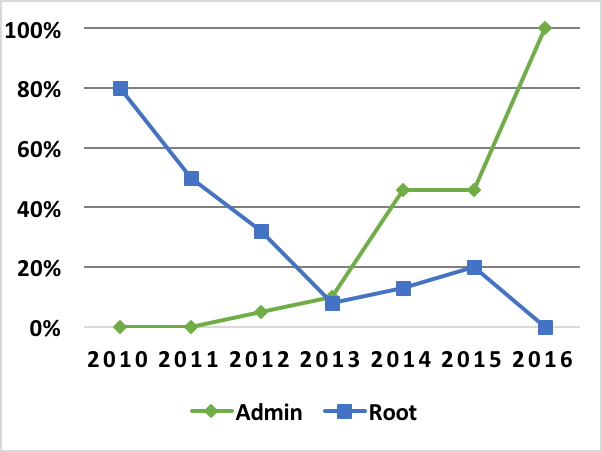
\includegraphics[width=0.9\linewidth]{fig/charts/pri.png}
  \caption{Privilege}
  \label{fig:sub:pri}
\end{subfigure}%
\begin{subfigure}[b]{.32\textwidth}
  \centering
  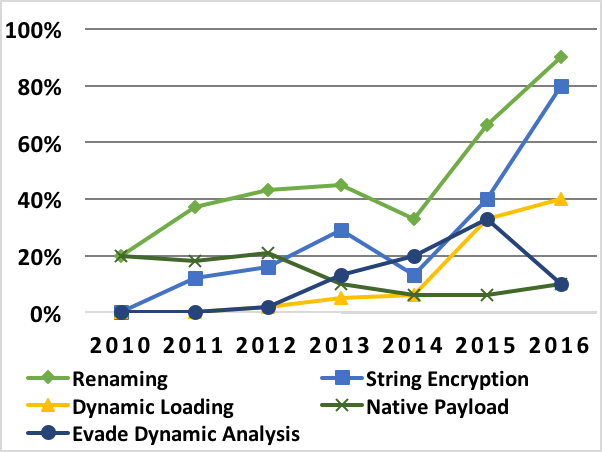
\includegraphics[width=0.9\linewidth]{fig/charts/anti.png}
  \caption{Anti-analysis}
  \label{fig:sub:anti}
\end{subfigure}%
\begin{subfigure}[b]{.32\textwidth}
  \centering
  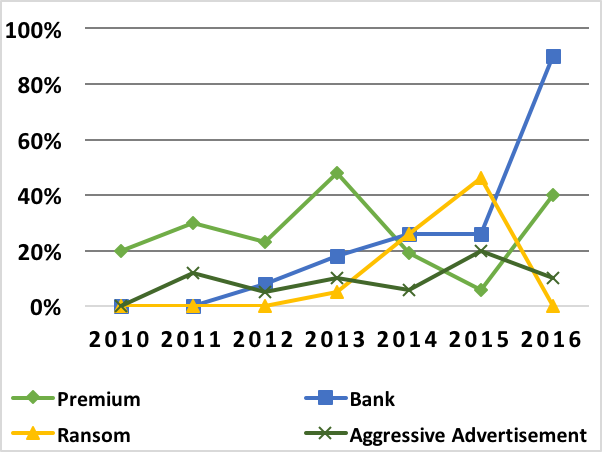
\includegraphics[width=0.9\linewidth]{fig/charts/mone.png}
  \caption{Monetizing}
  \label{fig:sub:mono}
\end{subfigure}
\caption{Malware Behavior Trends %. X axis represents the year from 2010 to 2016 whereas 
% (Y axis shows percentage within the year)  of malware variants appearing within the year
% having a particular behavior.
}
\vspace{-.25in}
\label{fig:behaviorcharts}
\end{figure}

We have performed a longitudinal study of our malware dataset with an attempt
to discover the trend of malware behaviors and techniques used over the years
from 2010 to 2016. For each type of behaviors and techniques, 
we observe the trend in terms of percentage of malware varieties manifesting a specific 
behavior/technique within a year.
%  requesting device-admin-privilege compared to percentage of malwares
% with root-exploit over the years).
Figure~\ref{fig:behaviorcharts} presents the results.
% evolution trace of the malware behavior and techniques.

Figure~\ref{fig:sub:ins} shows that the repackaging usage was growing until 2012,
but later standalone malware became dominant. The reason could be that
there are many effective anti-repackaging solutions made available during the last few years, 
which gives cybercriminals less incentive to use such techniques.
On the other hand, the bad guys are putting more effort into designing comprehensive
and sophisticated malware apps from scratch, and their malware design skill has matured. 

Not surprising to see in Figure~\ref{fig:sub:act} that listening to system events to
activate malware's functional units is the main trick given the nature of Android system design.
%Activation via host app comes along with repackaging or adware as expected.
Scheduling a task to periodically start its functional unit is an alarmingly growing trend.
By scheduling timer task or leveraging the {\em AlarmManager} the malware can constantly
upload victim's information to or retrieve commands from the C\&C server;
in the ransomware apps, it is also one of the techniques to lock victim's device.

We observe that persistence has become a core feature of Android malware apps. 
Figure~\ref{fig:sub:per} shows that malware apps are evolving to be harder 
to notice by the victim, % as they are hiding their appearance and hiding or cleaning the evidence.
and harder to be destroyed by the system,
anti-virus solutions, or users.

Root exploit is becoming less popular as we have discussed in Section~\ref{sec:profile:behavior:privilege},
but obtaining device-admin-privilege seems to have become popular as seen in Figure~\ref{fig:sub:pri}.
% We think that is because admin-privilege not only makes it harder to be uninstalled,
% but also can give cybercriminals the power to threat the victim user that her
% data is in danger.

The anti-analysis techniques are one of the key weapons of cybercriminals in 
the battle against security analysts.
From Figure~\ref{fig:sub:anti} we can see that renaming and string encryption
are the most growing techniques;
dynamic loading and evading dynamic analysis are catching up while
the practice of hiding behaviors in native payload is staying at the similar level.

Figure~\ref{fig:sub:mono} shows that banking malware is becoming the 
main channel for cybercriminals to make money.
% This is because people's banking behaviors are migrating from the
% PC world to the mobile phones, and more and more financial related activities are becoming available on mobile devices.
%Subscribe to premium service remains the same over the years.
Ransomware is a new threat that has started an uptick.

%%% Local Variables: 
%%% mode: latex
%%% TeX-master: "paper"
%%% End: 
